\documentclass[11pt]{memoir}

% 1st version for FASP 0.9.1 by Chensong Zhang
% 2nd version for FASP 1.3.5 by Chensong Zhang
% 3rd version for FASP 1.8.2 by Chensong Zhang and Ludmil Zikatanov

\usepackage[top=1in, bottom=1.5in, left=1in, right=1in]{geometry}
%\usepackage[notcite,notref,color]{showkeys}

\usepackage[pdftex,colorlinks=true,citecolor=blue,linkcolor=blue]{hyperref}
\usepackage{latexsym}
\usepackage{amsfonts}
\usepackage{amssymb}
\usepackage{amsmath}
\usepackage{url}
\usepackage{color}
\usepackage{graphicx}
\usepackage{epstopdf}
\DeclareGraphicsRule{.tif}{png}{.png}{`convert #1 `dirname #1`/`basename #1 .tif`.png}

% Define the listings environment
\usepackage{listings}
\usepackage{textcomp}
\definecolor{listinggray}{gray}{0.95}
\definecolor{lbcolor}{rgb}{0.9,0.9,0.9}
\lstset{
        numbers=left,
        numberstyle=\tiny,
        stepnumber=1,
        	backgroundcolor=\color{listinggray},
	tabsize=4,
	rulecolor=,
	language=C,
        basicstyle=\scriptsize,
        upquote=true,
        aboveskip={1.0\baselineskip},
        columns=fixed,
        showstringspaces=false,
        extendedchars=true,
        breaklines=true,
        prebreak = \raisebox{0ex}[0ex][0ex]{\ensuremath{\hookleftarrow}},
        frame=single,
        showtabs=false,
        showspaces=false,
        showstringspaces=false,
        identifierstyle=\ttfamily,
        keywordstyle=\bfseries\ttfamily\color[rgb]{0,0,1},
        commentstyle=\ttfamily\color[rgb]{0.1,0.6,0.2},
        stringstyle=\ttfamily\color[rgb]{1,0.1,0.3},
        linewidth=0.97\linewidth,
        xleftmargin=18pt,
}

% Define the frame environment
\usepackage{frame}
%\definecolor{shadecolor}{rgb}{1,0.9,0.1}
%definecolor{shadecolor}{RGB}{200,240,255}
\definecolor{shadecolor}{RGB}{255,240,200}

%%%%%%%%%%%%%%%%%%%%%%%%%%%%%%
\newtheorem{theorem}{Theorem}[section]
\newtheorem{definition}[theorem]{Definition}
\newtheorem{algorithm}[theorem]{Algorithm}
\newtheorem{example}[theorem]{Example}
\newtheorem{remark}[theorem]{Remark}
%%%%%%%%%%%%%%%%%%%%%%%%%%%%%%

\linespread{1.2}

\title{\Huge FASP User Guide}

\author{Chunsheng Feng, Xiaozhe Hu, Zheng Li, Jinchao Xu, \\
Chen-Song Zhang, Hongxuan Zhang, Ludmil Zikatanov}

\date{\vfill Version 1.8.2} % Activate to display a given date or no date

\begin{document}

\clearpage\maketitle
\thispagestyle{empty}

\newpage
\setcounter{page}{1}
\tableofcontents

%%%%%%%%%%%%%%%%%%%%%%%%%%%%%%
\chapter{Introduction}\label{ch:intro}
%%%%%%%%%%%%%%%%%%%%%%%%%%%%%%

% %%%%%%%%%%%%%%%%%%%%%%%%%%%%%%
% \section{What is FASP}\label{sec:goal}
% %%%%%%%%%%%%%%%%%%%%%%%%%%%%%%

% Over the last few decades, researchers have expended significant
% effort on developing efficient iterative methods for solving
% discretized partial differential equations (PDEs). Though these
% efforts have yielded many mathematically optimal solvers such as the
% multigrid method, the unfortunate reality is that multigrid methods
% have not been much used in practical applications. This marked gap
% between theory and practice is mainly due to the fragility of
% traditional multigrid (MG) methodology and the complexity of its
% implementation. We aim to develop techniques and the corresponding
% software that will narrow this gap, specifically by developing
% mathematically optimal solvers that are robust and easy to use in
% practice.

% We believe that there is no one-size-for-all solution method for
% discrete linear systems from different applications. And, efficient
% iterative solvers can be constructed by taking the properties of
% partial differential equations (PDEs) and discretizations into
% account. In this project, we plan to construct a pool of discrete
% problems arising from systems of PDEs and efficient linear solvers for
% these problems. We mainly utilize the methodology of Auxiliary Space
% Preconditioning (ASP) ~\cite{Xu.Xu.2010ff} to construct efficient
% linear solvers. Due to this reason, this software package is called
% ``Fast Auxiliary Space Preconditioning'' or FASP for short. 

\section{General description}
The Fast Auxiliary Space Preconditioning (FASP) package provides
C source files\footnote{The code is in the C99 (ISO/IEC 9899:1999) compatible.} to build a library of
iterative solvers and preconditioners for the solution of large-scale
linear systems of equations.  The components of the FASP basic library
include several ready-to-use, modern, and efficient iterative solvers
used in applications ranging from simple examples of discretized
scalar partial differential equations (PDEs) to numerical simulations
of complex, multicomponent physical systems via the Auxiliary Space
Preconditioning framework~\cite{Xu.Xu.2010ff}.

The main components of the FASP basic library are:
\begin{itemize}\setlength{\itemsep}{-1mm}
\item Basic linear iterative methods;
\item Standard Krylov subspace methods;
\item Geometric and Algebraic Multigrid (G/AMG) methods;
\item Incomplete factorization methods.
\end{itemize}
The FASP distribution also includes several examples for solving
simple benchmark problems.
%
The basic (kernel) FASP distribution is
open-source and is licensed under GNU Lesser General Public License or
LGPL. Other distributions may have different licensing (contact the
developer team for details on this).
%
\begin{snugshade}\noindent
  LICENSING: This software is free software distributed under the Lesser
  General Public License or LGPL, version~3.0 or any later
  versions. This software distributed in the hope that it will be
  useful, but WITHOUT ANY WARRANTY; without even the implied warranty
  of MERCHANTABILITY or FITNESS FOR A PARTICULAR PURPOSE. See the GNU
  Lesser General Public License \url{http://www.gnu.org/licenses/} for
  more details.
\end{snugshade}

\section{Roadmap: from basics to complex applications} 
A distinct feature of the FASP software project is that it is an open
ended project. It contains a basic kernel of sources and is maintained
by a team of developers with the expertise to build efficient solvers
for a wide range of complex numerical models.

As typical for an open-source software, the further development of
FASP project will also be based on the involvement of the community.
While we have our own plans for expanding FASP's capabilities, we also
count on the users' input in providing requests for, as well as,
contributions to, the expansion of FASP in different application
areas. Our team is ready to provide (or help with) the design and the
implementation of efficient solvers based on the FASP kernel to best
meet the goals and the requirements of our users.

The FASP software has been successfully used to build efficient
solvers for several discretized PDEs and systems of PDEs: general
scalar elliptic equations; linear elasticity; Brinkman equation;
bi-harmonic equation; Stokes and Navier-Stokes equations;
$H(\operatorname{curl})/H(\operatorname{div})$ systems; Maxwell's
system. The resulting solvers have been applied in simulations from
fluid dynamics, underground water simulation, fluid-structure
interactions, Oldryod-B and Johnson-Segalman models, black-oil model,
and magnetohydrodynamics (MHD).

Several of these benchmark problems are included as examples in
the open-source distribution, others are under development or have
more restrictive licensing.

%

% \begin{snugshade}\noindent
% We intend to design solution algorithms and their implementation for all these problems with different discretizations. We have done a bunch of them but not all of them are publicly available in the current version!
% \end{snugshade}


% FASP contains a kernel part and several example applications (ranging from
% fluid dynamics to reservoir simulation). The kernel part is
% open-source and licensed under GNU Lesser General Public License or
% LGPL. We tried and will continue to try to keep as many parts of the
% FASP project open to public as possible. However, some of the
% applications contain contributions from and owned partially by other
% parties. We only discuss the kernel functions (open to public) in this
% user's guide.


% \subsection{Our strategy}

% We organize the development of FASP package in a \emph{``Multilevel''} or \emph{``Capitalism''} way:

% \begin{itemize}

% \item Stage 1. Fine level stage (or free market stage)

% \begin{enumerate}
% \item[(1)] Collect problems and solvers. Allow similarities or even duplications, for example same solution algorithm, but different implementation. Keep all the record: problem description, solver code, test results, etc.
% %
% \item[(2)] Try to find a minimal set of standard or rules. And then we let the market to evolve freely. The idea is to allow the market to be FREE.
% \end{enumerate}

% \item Stage 2. Coarse level stage (or state capitalism stage)

% \begin{enumerate}
% \item[(1)] As FASP evolves, we might see, at certain time, that the market is out-of-control. This basically means the ``fine level solver'' or the ``free market'' is very successful and we should start to give more strict standard or regulation.
% %
% \item[(2)] Write a professional-level software package for a set of chosen algorithms for particular problems.
% \end{enumerate}
% \end{itemize}
%%%%%%%%%%%%%%%%%%%%%%%%%%%%%%
\section{How to use this guide}\label{sec:how}
%%%%%%%%%%%%%%%%%%%%%%%%%%%%%%

This user's guide describes how to use the existing solvers in FASP
via a couple of simple tutorial problems. The user's guide is a
self-contained document but does \emph{not} provide any details about
the algorithms or their implementation. Along with this guide, we provide a
reference manual\footnote{Available online at
  \url{http://fasp.sourceforge.net}. It is also available in
  ``\url{faspsolver/doc/doc.zip}''.} for technical details on the
implementation which includes references. We recommend that the users
read these references to better
understanding of the code. Furthermore, since FASP is under heavy
development, please use this guide with caution because the code might
have been changed before this document is updated.


%%%%%%%%%%%%%%%%%%%%%%%%%%%%%%
\section{How to obtain FASP}\label{sec:install}
%%%%%%%%%%%%%%%%%%%%%%%%%%%%%%

There are several ways to download the FASP source files. We recommend users download the most updated version from the FASP page on SourceForge. 

\subsection{Downloading from SourceForge}

The most updated version of FASP can be downloaded directly from
%
\begin{center}
\url{http://fasp.sf.net/download/faspsolver.zip}
\end{center}
%

\subsection{Downloading from BitBucket}

FASP is also hosted on
\emph{BitBucket.org}\footnote{Official website:
  \url{https://bitbucket.org/}} using Mercurial (Hg)\footnote{Official
  website: \url{http://mercurial.selenic.com/}}. A Hg client for GNU
Linux, Mac OS X, or Windows can be downloaded from
% section section name (end)
\begin{center}
  \url{http://mercurial.selenic.com/downloads/}
\end{center}
%
There are also many other third-party clients which provides Hg services, for example: EasyMercurial\footnote{Official website: \url{http://easyhg.org}} (cross platform) and SourceTree\footnote{Official website: \url{http://www.sourcetreeapp.com}} (for Mac OS X only).

As a DVCS (Distributed Version Control System) source-control
software, Hg is relatively new. But compared with other tools like
Git, Hg is considered \emph{friendlier} with a lower learning
curve. This is despite the fact that Hg uses two distinct sets of
commands and two distinct vocabularies for operations depending upon
whether the repository is local or remote.  Documentation for Hg is
substantially better, including a book\footnote{The hgbook,
  \url{http://hgbook.red-bean.com/}}. They've also had the advantage
of trying the documentation on a fairly savvy group of developers
(Mozilla) who gave them lots of feedback that helped polish the rough
edges.

\subsection{Linux or Mac OS X}
First, you need to obtain a free copy of FASP kernel functions from
our public Hg repository. If you are downloading FASP for the first
time, you can clone the repository to your local machine:
%
\begin{lstlisting}[numbers=none]
"Download FASP kernel subroutines via HTTPS"

$ hg clone https://faspusers@bitbucket.org/fasp/faspsolver
\end{lstlisting}
%
\begin{snugshade}\noindent
If you have any problems when clone this repository, please send us an email to \url{faspdev@gmail.com}.
\end{snugshade}

After a long pause\footnote{In fact, a very long pause. This is
  because the initial clone with copy all the history data which is
  about 400MB in total. Depending on the speed of your network, it
  could take 15 minutes to one hour.}, you should have obtained
``\emph{faspsolver}'' in your current directory successfully. If you
have already cloned the repository before, you can just pull a new
version and update your local version with it: Go to your local
``\emph{faspsolver}'' directory and then
%
\begin{lstlisting}[numbers=none]
"Pull a new version from BitBucket"
$ hg pull

"Update you local version to the new version"
$ hg update
\end{lstlisting}
%

\subsection{Windows OS}
If you are using Windows, you may want to install
TortoiseHg\footnote{Official website:
  \url{http://tortoisehg.bitbucket.org/}}. After installing it, the
TortoiseHg menu has been merged into the right-click menu of Windows
Explore. You could download FASP copy from BitBucket.org. Choose
``TortoiseHg''\verb| --> |``Clone'' in the pop-up menu, the source
address is
\begin{center}
\url{https://faspusers@bitbucket.org/fasp/faspsovler}
\end{center}
Then press ``Clone'' and you will obtain ``faspsolver'' in the directory you set.


\section{Building and installing the FASP library and examples}\label{sec:build}

FASP has been tested using the compilers and built-in libraries of
several Linux distributions (\verb|Cent OS|, \verb|Debian|,
\verb|Fedora|, \verb|RedHat|, \verb|Ubuntu|) Mac OS X 10.6 and later
(Leopard, Snow Leopard, Lion, Mavericks, Yosemite, El Capitan), and
Windows (XP, Win 7) with several compliers, including \verb|gcc|,
\verb|g++|, \verb|clang|, \verb|icc|, \verb|VC++|. FASP also easily
links to applications written in Fortran and this has been tested with
\verb|gfortran|, \verb|g95|, \verb|ifort| Fortran compilers.

\subsection{FASP on Linux or Mac OS X}
To build the FASP library for these operating systems. Open a terminal
window, wehre you can issue commands from the command line and do the following: 
(1) go to the main FASP directory (we will refer to it as
\verb|$(faspsolver)| from now on); (2) modify the ``\emph{FASP.mk.example}''
file to math your system and save it as ``{\color{red}FASP.mk}''; (3) then execute:
%
\begin{lstlisting}[numbers=none]
$ make config 
$ make install
\end{lstlisting}
%
These two commands build the FASP library/header files. It installs
the library in \verb|$(faspsolver)/lib|
and the header files in \verb|$(faspsolver)/include|. It also creates a
file \verb|$(faspsolver)/Config.mk| which contains few of the configuration
variables and can be loaded by external project Makefiles (see
\S\ref{sec:buildown} for details on \verb|$(faspsolver)Config.mk|).

If you do not have ``FASP.mk'' present in the current directory,
default settings will be used for building and installation FASP. 

Next, if you would like to try some of the examples that come with
FASP, you can build the ``test'' and ``tutorial'' targets as follows:
%
\begin{lstlisting}[numbers=none]
$ make test
$ make tutorial
\end{lstlisting}
%
Equivalently, you may also build the test suite and the tutorial examples by using
the ``local'' Makefile(s) in \verb|$(faspsolver)/test|
and \verb|$(faspsolver)/tutorial|.
\begin{lstlisting}[numbers=none]
$ make -C test
$ make -C tutorial
\end{lstlisting}

\begin{snugshade}
  \noindent
  Note: While these two approaches to build the FASP test suite and the
  FASP examples
  produce equivalent result in most cases, we note an important
  difference. The former approach uses a
  \verb|CMake| installation process. The latter works without invoking
  \verb|Cmake| and represents an example of how one may link
  an external project with the FASP library. We refer to
  \S\ref{sec:buildown} below for more details. 
\end{snugshade}

If everything went all right, you can go to the
``\url{faspsolver/test}'' directory and try to run a test problem:
%
\begin{lstlisting}[numbers=none]
$ ./test.ex
\end{lstlisting}
%
If you need help with the available options, type 
%
\begin{lstlisting}[numbers=none]
$ make help
\end{lstlisting}
%
and you will get the following screen
\lstinputlisting[numbers=none,language=sh]{../INSTALL}

Many options can be changed in "FASP.mk", as well as from the command
line. For example,
\begin{lstlisting}[numbers=none]
$ make config CC=gcc49 prefix=/usr/local
$ sudo make install
\end{lstlisting}
will install in the FASP library in \verb|/usr/local/lib| and the
include files in \verb|/usr/local/include| so that they may be
accessed by multiple users.

\begin{snugshade}\noindent
  The example given above in most cases will require administrative
  privileges from the user, i.e. using \verb|sudo| or other equivalent
  mechanism, to install in a system directory (such as
  \verb|/usr/local| in our example). We do not recommend such way of
  installing FASP, although it will work in most cases if the user has
  administrative privileges.  We recommend installation of FASP
  library/headers locally and then, if needed, copying them to a
  different location.
\end{snugshade}

To uninstall FASP and clean up the working directory, you can run
%
\begin{lstlisting}[numbers=none]
$ make uninstall
$ make distclean
\end{lstlisting}
%

\subsection{Windows 7}

We provide a Visual Studio 2008 (VS08) distribution and a VS10
distribution of FASP for Windows users. For example, you can just open
``\url{faspsolver/vs08/faspsolver-vs08.sln}'' if you are using VS08 as
your default developing environment. Then a single-click at the
``Build Solution'' on the menu or ``F7'' key will give you all the
FASP libraries and the test programs in
``\url{faspsolver/test/}''. The way for building in VS10 is similar.
\begin{figure}[htbp] %  figure placement: here, top, bottom, or page
   \centering
   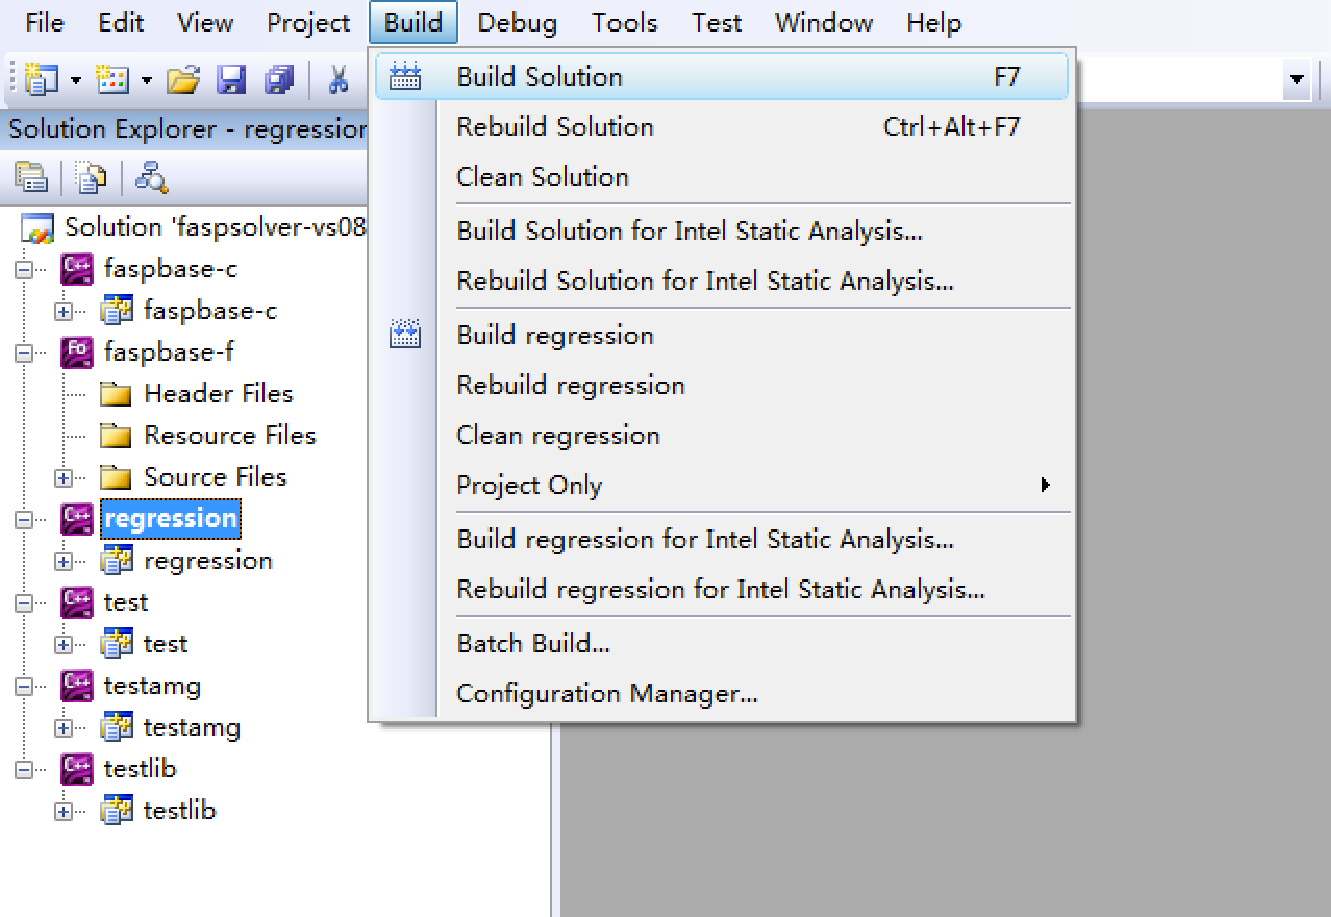
\includegraphics[width=\linewidth]{fig/build-fasp-win7.pdf} 
   \caption{Build FASP using Visual Studio 2008.}
   \label{fig:build}
\end{figure}

\begin{snugshade}\noindent
  You need a C/C++ complier and the Visual Studio to build FASP. For
  example, the build can be accomplished using either Microsoft Visual
  C++ or Intel C compiler. %together with Intel Fortran compiler.
\end{snugshade}

\begin{snugshade}\noindent
  If you are using other versions of Visual Studio (like VS05 or
  VS12), we advise NOT to convert the ``VS08'' files to your newer VS version
  automatically because the FASP source files might be {\color{red}removed} by the
  Visual Studio. In such a case, we recommend that you
  create your own version to build all the libraries and test
  programs.
\end{snugshade}

If you need to build a VS FASP yourself, you need to create 5 projects:
\begin{enumerate}
\item ``faspbase-c'' contains all the ``.c'' and ``.inl'' files in the
  directory ``./base/src/''. You should add ``./base/include'' in
  Additional Directories. This project contains the core subroutines
  of faspsolver.
\item ``faspbase-f'' contains all the ``.f'' files in
  ``./base/extra/sparsekit''.
\item ``testlib'' contains all the ``.c'' files in
  ``./test/src/''. You should add ``./test/include'' in Additional
  Directories.
\item ``test'' is an executing program for test purpose in FASP. The
  source file is ``./test/main/test.c''.
\item ``regression'' is another executing program, which contains
  several methods to test the problems. The source file is
  ``./test/main/regression.c''.
\end{enumerate}

\begin{snugshade}\noindent
  NOTE: If you are using Visual C++, all the C files should be
  compiled as C++ code (by using the /TP compiling option).
\end{snugshade}

After a successful build on VS, you will have two static libraries
named ``faspbase-c-vs08.lib'' and ``faspbase-f-vs08.lib''. You can use
the ``lib'' command to wrap them together as one single file
(e.g. FASP.lib) for better portability. For example:
%
\begin{lstlisting}[numbers=none]
C:\FASP> lib /ltcg /out:FASP.lib faspbase-c-vs08.lib faspbase-f-vs08.lib
\end{lstlisting}
%

\subsection{Using a TCL based GUI for installation}
For users who like more a GUI based installation, we provide a simple
TCL Graphical User
Interface (GUI) for building the FASP library. On a machine running
Linux or Mac OS X with \verb|Tcl/Tk| installed, you may invoke the GUI
by typing
%
\begin{lstlisting}[numbers=none]
$ wish FASP_install.tcl
\end{lstlisting}
%
\begin{figure}[h!!] %  figure placement: here, top, bottom, or page
   \centering
   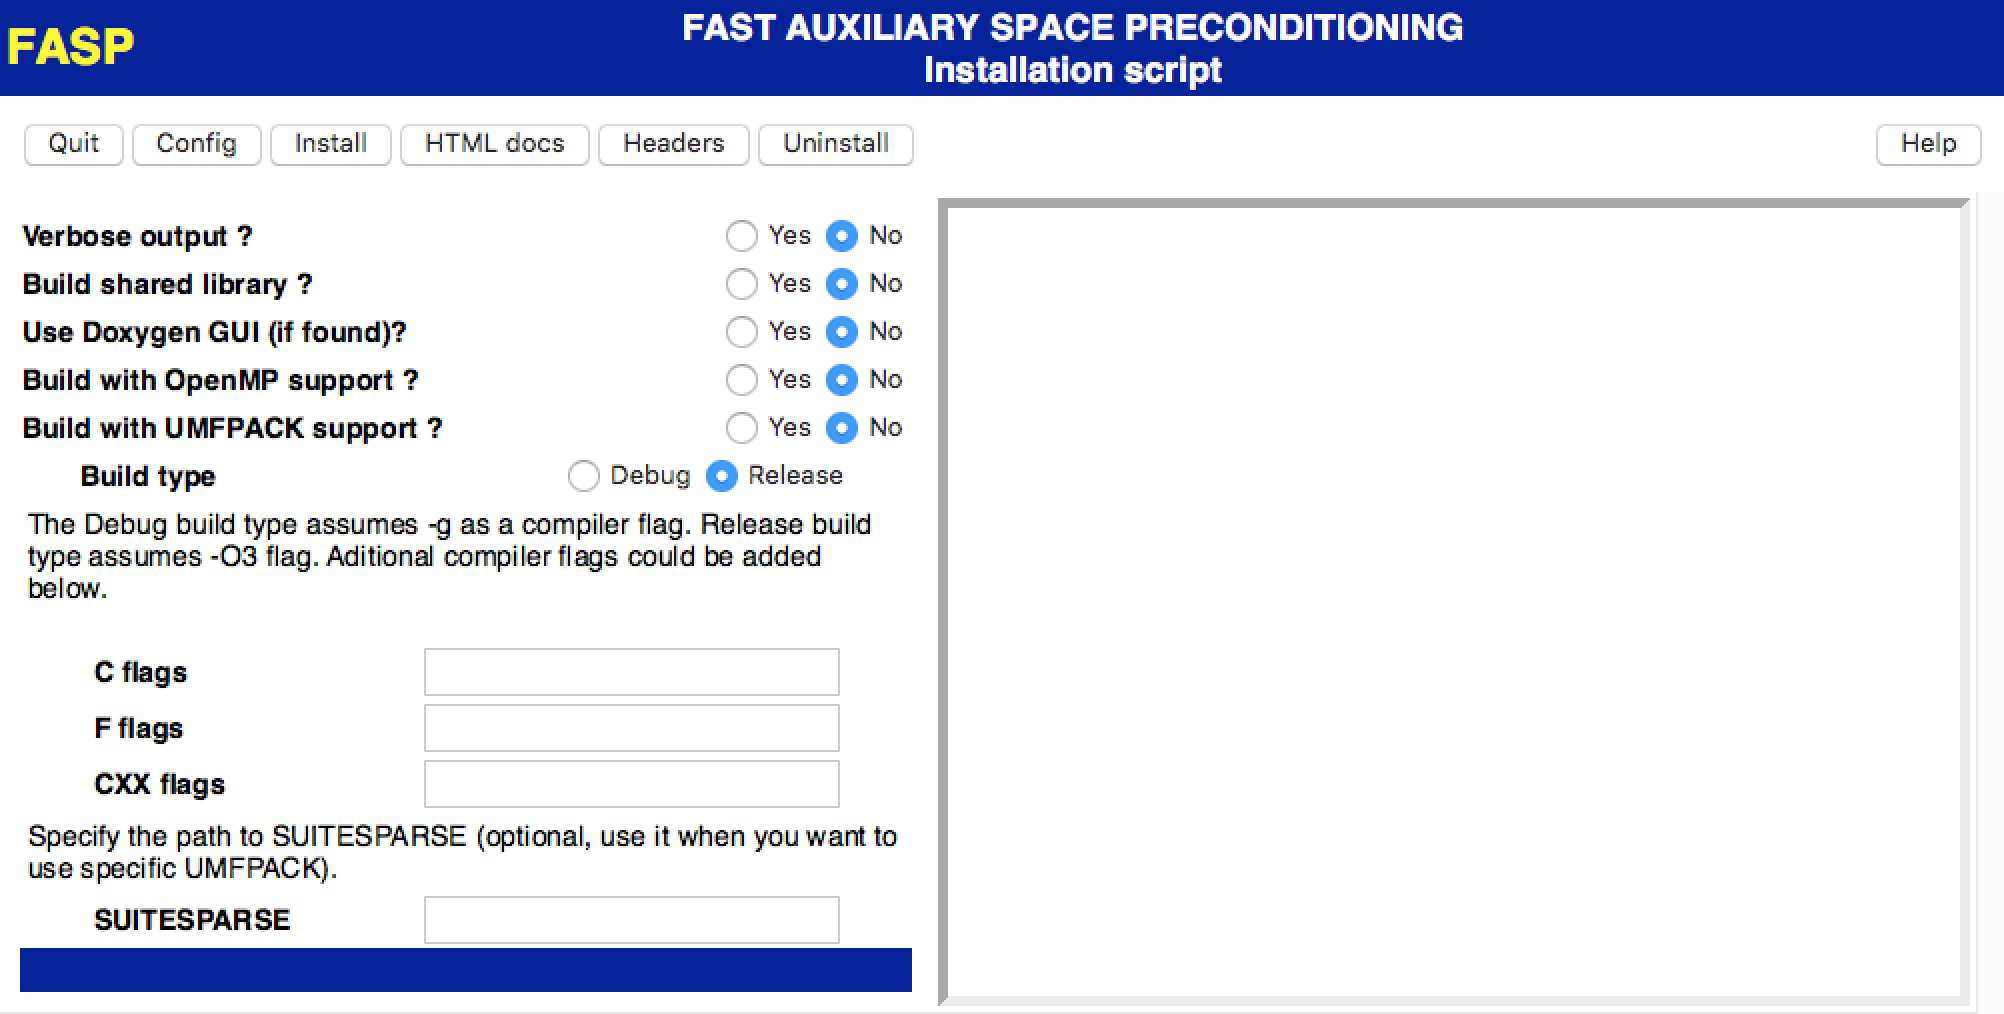
\includegraphics[width=\linewidth]{fig/install-fasp-gui.png} 
   \caption{Install FASP using the TCL GUI on Mac OS X El Capitan.}
   \label{fig:gui}
\end{figure}
%
If all is OK, you should see on your screen the FASP window as shown
in Figure~\ref{fig:gui}. The rest of the building process is more or
less straightforward: After choosing appropriate parameters, click
``Config'' first, followed by clicking ``Install''.

\begin{comment}
\subsection{Using Scons}
Another possibility for building FASP is to use the \verb|python|
based Scons interface for Linux, Mac OS X, or Windows, 
and install different versions (Release, Shared, Debug) of the FASP
library. To use Scons, change the working directory to
``\url{faspsolver/base}'' and type:
%
\begin{lstlisting}[numbers=none]
$ scons -Q install
\end{lstlisting}

By default, Scons will search for default compilers installed on your
system. If you wish to use a specific compiler, you may change the
default values of the CC (for C) and FC (for Fortran) flags. For
in a Windows environment in order to use the Intel Fortran and VC++
compilers for FASP, the Scons command is:
\begin{lstlisting}[numbers=none]
C:\> scons -Q install FC=ifort CC=cl
\end{lstlisting}

\begin{snugshade}\noindent
  In many cases the directories where additional compilers reside are
  not automatically added to the PATH environment variable
  automatically. Hence, you may need to modify your PATH variable to
  make the command above to work.
\end{snugshade}
\end{comment}


\subsection{External libraries}\label{ssec:lib}

There are a few \emph{optional} external libraries that you might want
to use, including memory allocation routines, direct solvers, ILU
methods, discretization packages, etc. FASP has interfaces to several
of them, for example, FASP can be linked to use \verb|UMFPack|, \verb|SuperLU|, \verb|MUMPS|,
\verb|SparseKit|, \verb|dlmalloc|.


\section{Linking your own project with FASP}\label{sec:buildown}
The FASP distribution comes with two ``local'' Makefile(s) in the
sub-directories for ``test'' and ``tutorial'', namely,
\verb|$(faspsolver)/test/Makefile| and
\verb|$(faspsolver)/tutorial/Makefile|.
These two makefiles can be used to build the FASP tests and tutorial
examples. They use minimal information about the library built. For
convenience, at configuration time, such information is stored in
\verb|$(faspsolver)/Config.mk| file for later use. A typical contents
of such file is given below:
\begin{lstlisting}[language=sh,numbers=none]
########################### Automatically generated ###################
# Fast Auxiliary Space Preconditioners (FASP) 
#
#######################################################################
# This file is rewritten when "make config" is run.
# It is (s)included by test/Makefile and tutorial/Makefile
#
#######################################################################
fasp_prefix=/path/to/faspsolver
fasp_library=libfasp.a
CC=gcc
CXX=g++
FC=gfortran
#######################################################################
\end{lstlisting}
The variables defined in this file can also be set directly in
\verb|$(faspsolver)/test/Makefile|,
\verb|$(faspsolver)/tutorial/Makefile|, or, in your own Makefile. An
external project can be compiled and linked with FASP by following the
rules set in \verb|$(faspsolver)/tutorial/Makefile| (included below):
\lstinputlisting[language=sh]{../tutorial/Makefile}

%%%%%%%%%%%%%%%%%%%%%%%%%%%%%%
\chapter{A brief tutorial}\label{ch:tutor}
%%%%%%%%%%%%%%%%%%%%%%%%%%%%%%

In this chapter, we discuss several simple examples included with this
FASP distribution and demonstrating how to
use the FASP package for solving linear systems. We read the matrices
from disk files (the files are also included in the FASP
distribution). 
All the examples in this section can be found inside ``\url{faspsolver/tutorial/}''. 

After you successfully build FASP (see \S\ref{sec:build}), just go to the
``\url{faspsolver/tutorial/}" directory and the tutorial
examples should be ready to run.

In this section we mainly discuss the C version of these examples; the FASP
distribution also includes F90 versions of some of the examples. 

\begin{snugshade}\noindent 
  In the description below, we display a typical output from runs of
  each of the examples.  Note that the actual output depends on the
  solver parameters, and, on your computer it may be be different than
  what you see here.
\end{snugshade}

\newcounter{ex}
\setcounter{ex}{1}

%%%%%%%%%%%%%%%%%%%%%%%%%%%%%%
\section{Example \arabic{ex}: An AMG solver for the Poisson equation}\label{sec:ex1}
%%%%%%%%%%%%%%%%%%%%%%%%%%%%%%
\addtocounter{ex}{1}

The first example is a standard one: We read a symmetric
positive definite matrix $A$ and right-hand side $b$ from harddisk and then we solve
$Ax=b$ using the classical AMG
method~\cite{Brandt.BrandtMcCormick.1982uq,Ruge.RugeStuben.1985ij,Ruge.RugeStuben.1987bs};
see \S\ref{sec:amg}. In this example the matrix $A$ included with the
FASP distribution corresponds to a discretization with continuous
piecewise linear finite elements of the Poisson equation
$$-\Delta u = f$$ (with the Dirichlet boundary conditions) on a
triangulation of a bounded domain $\Omega$.
%
\lstinputlisting[language=C]{../tutorial/main/poisson-amg.c}
%
Since this is the first example, we will explain it in some detail:
\begin{itemize}
%
\item Line 1 tells the Doxygen documentation system\footnote{Doxygen \url{http://www.doxygen.org} is a useful tool for generating documentation from annotated sources. We use it in FASP development.} that the filename
  is ``\verb|poisson-amg.c|''. Line 3--5 tells the Doxygen what is the
  purpose of this file (function).
%
\item Line 12--13 includes the main FASP header file ``\verb|fasp.h|'' and
  FASP function declarations header ``\verb|fasp_functs.h|''. These two
  headers shall be included in all files that requires FASP
  subroutines. Please also be noted that the function declarations in
  ``\verb|fasp_functs.h|'' are automatically generated from the source files
  by an \verb|awk| script and we do not recommend modifying this file,
  since your changes may be lost. 
%
\item Line 35--36 sets solver parameters using the default parameters or
  from the command line options; see more discussions in
  \S\ref{sec:parameters}. In the ``\verb|tutorial/ini/amg.dat|'' file, we can
  set the location of the data files, type of solvers, maximal number
  of iteration numbers, convergence tolerance, and many other
  parameters for iterative solvers.
%
\item Line 44 defines a sparse matrix $A$ in the compressed sparse row
  (CSR) format. Line 45 defines two vectors: the right-hand side $b$
  and the numerical solution $x$. We refer to~\S\ref{sec:blas} for
  definitions of vectors and general sparse matrices.
%
\item Line 57 reads the matrix and the right-hand side from two disk
  files. Line 46--55 defines the filenames of them.
%
\item Line 60--64 prints basic information of coefficient matrix,
  right-hand side, and solver parameters.
%
\item Line 69--70 allocates memory for the solution vector $x$ and set
  its initial value to be all zero.
%
\item Line 72 solves $Ax=b$ using the AMG method. Type of the AMG
  method and other parameters have been given in ``\verb|amgparam|'' at Line
  36; see \S\ref{sec:amg}.
%
\item Line 75--77 frees up memory allocated for $A$, $b$, and $x$.
\end{itemize}
%
To run this example, type:
%
\begin{lstlisting}[numbers=none]
$ ./poisson-amg-c.ex
\end{lstlisting}
%
A sample output is listed as follows:
%
\lstinputlisting[numbers=none,firstline=2]{../tutorial/out/poisson-amg-c.out}

We also provide a Fortran 90 example, which does the same thing as
this C code except it gives less output, in
``\url{tutorial/main/poisson-amg.f90}''. Users who would like to call
FASP solver from a Fortran based application can see how to do this example.
%
\lstinputlisting[language=Fortran]{../tutorial/main/poisson-amg.f90}
%

%%%%%%%%%%%%%%%%%%%%%%%%%%%%%%
\section{Example \arabic{ex}: Conjugate gradient without preconditioning}\label{sec:ex2}
\addtocounter{ex}{1}
%%%%%%%%%%%%%%%%%%%%%%%%%%%%%%
In the second example, we modify the previous example slightly and
solve the Poisson equation using iterative methods (here by default we
use the Conjugate Gradient method without preconditioning).
%
\lstinputlisting[language=C]{../tutorial/main/poisson-its.c}
%
This example is very similar to the first example and we briefly explain the differences:
\begin{itemize}
%
\item Line 67--68 allocates memory for the solution vector $x$ and set its initial value to be all zero.
%
\item Line 70 solves $Ax=b$ using the general interface for Krylov subspace methods. Type the iterative method and other parameters have been specified in ``\verb|itparam|''; see \S\ref{sec:iter} for details.
%
\end{itemize}
%
To run this example, we can simply type:
%
\begin{lstlisting}[numbers=none,language=sh]
$ ./poisson-its-c.ex
\end{lstlisting}
%
A sample output is as follows:
\lstinputlisting[numbers=none,firstline=2,lastline=76]{../tutorial/out/poisson-its-c.out}

%%%%%%%%%%%%%%%%%%%%%%%%%%%%%%
\section{Example \arabic{ex}: Conjugate gradient with preconditioning}\label{sec:ex3}
%%%%%%%%%%%%%%%%%%%%%%%%%%%%%%
\addtocounter{ex}{1}

This example is a bit more involved and is a modification of the
previous one. In this example, we wish to demonstrate how to use a the
FASP library and run a preconditioned conjugate conjugate gradient (PCG) method.
%
\lstinputlisting{../tutorial/main/poisson-pcg.c}
%
This example is very similar to the first example, and the details are
as follows. 
\begin{itemize}
%
\item Line 36--37 sets default parameters. In this example, we need parameters for iterative methods, AMG preconditioner, and ILU preconditioner. 
%
\item Line 73 sets up the desired preconditioner and prepare it for the preconditioned iterative methods.
%
\item Line 83 calls PCG to solve $Ax=b$. One can also call the general iterative method interface as in the previous example.
%
\item Line 86 cleans up auxiliary data associated with the preconditioner in use if necessary. 
%
\end{itemize}
%
To run this example, we can simply type:
%
\begin{lstlisting}[numbers=none]
$ ./poisson-pcg-c.ex
\end{lstlisting}
%
A sample output is given as follows (note that the actual output depends on the solver parameters and might be different than what you see here):
\lstinputlisting[numbers=none,firstline=2]{../tutorial/out/poisson-pcg-c.out}

We also provide a Fortran 90 example, which does the same thing as
this C code except it gives less output, in
``\url{tutorial/main/poisson-pcg.f90}''. Users who would like to call
FASP solver from a Fortran based application can see how to do this example.
%
\lstinputlisting[language=Fortran]{../tutorial/main/poisson-pcg.f90}
%

%%%%%%%%%%%%%%%%%%%%%%%%%%%%%%
\section{Example \arabic{ex}: An GMG solver for the Poisson equation}\label{sec:ex4}
%%%%%%%%%%%%%%%%%%%%%%%%%%%%%%
\addtocounter{ex}{1}

The geometric multigrid method (GMG) is one of the most efficient solving techniques for discrete algebraic systems arising from many types of partial differential equations~\cite{Bramble.Bramble.1993fk,Trottenberg.TrottenbergOosterlee.2001fu}. GMG utilizes a hierarchy of grids or discretizations and reduces the error at a number of frequencies simultaneously. Because of its plausible linear complexity---i.e., the low computational cost of solving a linear system with $N$ unknowns is $O(N)$---the GMG method is one of the most popular Poisson solvers. Although the GMG's applicability is limited as it requires explicit information on the hierarchy of the discrete system, when it can be applied, GMG is far more efficient than its algebraic version, the algebraic multigrid (AMG) method.

We now give a simple example on calling the geometric multigrid for solving the Poisson's equation in 2D (discretized by the standard five-point finite difference stencil). Consider the Poisson equation
\begin{equation*}
\left\{
\begin{array}{rcl}
    - \Delta u &=&  f  \qquad \mbox{in }~\Omega \\
      u &=& 0  \qquad \mbox{on }\partial\Omega, \\
\end{array}
\right.
\end{equation*}
where $\Omega = (0,1)^2 \subset \mathbb{R}^2$.
%
The main reason why we choose this simplest possible setting is to emphasize that, even for a simple problem, the new heterogeneous architectures present challenges for numerical implementation. Another reason is to allow us to use explicit stencils and to avoid the bottleneck of sparse matrix-vector production. 
%
The standard central finite difference method is applied to discretize the Poisson's equation. In other words, the Laplace operator is discretized by the classical second-order central difference scheme. After discretization, we end up with a system of linear equations:
%
     \begin{equation*}
        \mathbf{A}\vec{u} = \vec{f}.
    \end{equation*}
%    
We use the five-point central difference scheme in 2D. Consider a uniform square mesh of $\Omega = [0, 1]^2$
with size $h = \frac{1}{n}$ and in which $x_i = ih, \, y_j = jh \, (i, j = 0,
1,\ldots, n)$. Let $u_{i,j}$ be the numerical approximation of $u(x_i , y_j )$. The five-point central
difference scheme for solving the Poisson's equation in 2D can be written as follows:
$$
{-u_{i-1,j}-u_{i,j-1}+4u_{i,j}-u_{i+1,j}-u_{i,j+1}}={h^2}f(x_i,y_j)
\qquad i, j=1,2,\ldots,n-1.
$$

The sample code for this solver can be found in ``\url{tutorial/main/poisson-gmg.c}'' and a piece of the source code is listed as follows:
%
\lstinputlisting[language=C]{../tutorial/main/poisson-gmg.c}
%

%%%%%%%%%%%%%%%%%%%%%%%%%%%%%%
\section{Example \arabic{ex}: Block ILU preconditioner}\label{sec:ex5}
%%%%%%%%%%%%%%%%%%%%%%%%%%%%%%
\addtocounter{ex}{1}

We now show a simple example for calling iterative solvers in BSR format. The test example is from a test problem given by the Society of Petroleum Engineers (SPE01 Benchmark) using a fully implicit black-oil simulator at certain time step. The test matrix is the Jacobian matrix from the Newton linearization and is stored as a BSR matrix (see~\S\ref{sec:bsr} for details). 

The sample code for this solver can be found in ``\url{tutorial/main/spe01-its.c}'' and a piece of the source code is listed as follows:
%
\lstinputlisting[language=C]{../tutorial/main/spe01-its.c}
%
A sample output is given as follows (note that the actual output depends on the solver parameters and might be different than what you see here):
\lstinputlisting[numbers=none,firstline=2]{../tutorial/out/spe01-its-c.out}

%%%%%%%%%%%%%%%%%%%%%%%%%%%%%%
\section{How to change parameters for
  solvers/preconditioners}\label{sec:parameters}
%%%%%%%%%%%%%%%%%%%%%%%%%%%%%%

In the previous examples, we have seen how to use the default parameters in FASP. In this section we discuss changing such parameters
by reading them from a disk file or from the command line. An example of parameter initialization file is found in the FASP
tutorial directory and is named ``\url{tutorial/ini/amg.dat}''.
%
\begin{lstlisting}[numbers=none,language=sh]
$ ./poisson-amg-c.ex -ini ini/amg.dat
\end{lstlisting}
%
We take ``\verb|tutorial/ini/amg.dat|'' as an example:
\lstinputlisting{../tutorial/ini/amg.dat}

We now briefly discuss the parameters above:
%
This example is very similar to the first example and we now briefly explain it:
\begin{itemize}
%
\item Line 7 sets the working directory, which should contain data files for the matrices (and right-hand side vectors when necessary).
%
\item Line 8 sets the level of output for FASP routines. It should range from 0 to 10 with 0 means no output and 10 means output everything possible.
%
\item Line 14--25 sets the basic parameters for multilevel iterations. For example, type of AMG, type of multilevel cycles, number of maximal levels, etc.
%
\item Line 31--38 sets the type of smoothers, number of smoothing sweeps, etc.
%
\item Line 44--50 sets the parameters for the setup phase of the classical AMG method (\S\ref{sec:amg}).
%
\item Line 56--59 gives the parameters for the setup phase of the aggregation-base AMG methods (\S\ref{sec:amg}).
%
\end{itemize}
%

You can do a very simple experiment---Simply change the AMG type from the classical AMG to smoothed aggregation AMG by revise Line 14 to:
%
\begin{lstlisting}[numbers=none]
AMG_type                 = SA
\end{lstlisting}
%
Then you run ``poisson-amg-c.ex'' one more time and will get
%
\lstinputlisting[numbers=none,firstline=2]{../tutorial/out/poisson-amg-c-sa.out}
%
You can compare this with the sample results in \S\ref{sec:ex1}.

\begin{snugshade}\noindent  
The input parameters allowed in FASP are not limited to the ones listed in this example. A list of possible iterative methods and preconditioners can be found in ``\verb|base/include/fasp_const.h|''; see \S\ref{sec:const}. For more parameters and their ranges, we refer to the FASP Reference Manual.
\end{snugshade}

Using ``-ini [FILE]'' is just one example of allowed command line option. To find out more what command line options are acceptable, you can type in a terminal window:
%
\begin{lstlisting}[numbers=none,language=sh]
$ ./poisson-amg-c.ex -help
\end{lstlisting}
%
which will give you something like
%
\begin{lstlisting}[numbers=none,language=sh]
========================================
||   FASP: AMG example -- C version   ||
========================================

FASP command line options:
================================================================
  -ini              [CharValue] : Ini file name
  -print            [IntValue]  : Print level
  -output           [IntValue]  : Output to screen or a log file
  -solver           [IntValue]  : Solver type
  -precond          [IntValue]  : Preconditioner type
  -maxit            [IntValue]  : Max number of iterations
  -tol              [RealValue] : Tolerance for iterative solvers
  -amgmaxit         [IntValue]  : Max number of AMG iterations
  -amgtol           [RealValue] : Tolerance for AMG methods
  -amgtype          [IntValue]  : AMG type
  -amgcycle         [IntValue]  : AMG cycle type
  -amgcoarsening    [IntValue]  : AMG coarsening type
  -amginterpolation [IntValue]  : AMG interpolation type
  -amgsmoother      [IntValue]  : AMG smoother type
  -amgsthreshold    [RealValue] : AMG strong threshold
  -amgscoupled      [RealValue] : AMG strong coupled threshold
  -help                         : Brief help messages
 \end{lstlisting}
%

For example, in order to the change the AMG type to the smoothed aggregation (SA) used by the preconditioner for PCG, you can also use the command line options:
%
\begin{lstlisting}[numbers=none,language=sh]
./poisson-amg-c.ex -amgtype 2 -amgmaxit 100
\end{lstlisting}
%
Here we only changed two parameters from the default setting without changing anything else. So it might not give the same output as in the previous example. 

%%%%%%%%%%%%%%%%%%%%%%%%%%%%%%
\chapter{Data structures and basic usage}\label{ch:basic}
%%%%%%%%%%%%%%%%%%%%%%%%%%%%%%

In this chapter, we discuss the basic data structures and the
important building blocks which are useful for constructing auxiliary
space preconditioners for systems of PDEs in
Chapter~\ref{ch:advanced}. In particular, we will discuss vectors,
sparse matrices, iterative methods, and multigrid methods.

%%%%%%%%%%%%%%%%%%%%%%%%%%%%%%
\section{Vectors and sparse matrices}\label{sec:blas}
%%%%%%%%%%%%%%%%%%%%%%%%%%%%%%

The data structures most often used for implementing iterative methods are
sparse matrices and vectors. In this section, we first discuss the
data structures for vectors and matrices in FASP; and then we discuss
BLAS operations for sparse matrices. The definitions can be found in
``\url{base/include/fasp.h}''.

\subsection{Vectors}

The data structure for vectors is very simple. It only contains the length of the vector and an array which contains the entries of this vector.
%
\lstinputlisting[language=C,firstnumber=330,firstline=330,lastline=342]{../base/include/fasp.h}
%

\subsection{Sparse matrices}

On the other hand, sparse matrices for PDE applications are very complicated. It depends on the particular applications, discretization methods, as well as solution algorithms. In FASP, there are several types of sparse matrices, COO, CSR, CSRL, BSR, and CSR Block, etc. The presentation closely follows ideas from Pissanetzky~\cite{Pissanetzky.Pissanetzky.1984hc}.

In this section, we use the following sparse matrix as an example to explain different formats for sparse matrices:
%
\begin{example}\label{ex:sparse}
Consider the following $4\times 5$ matrix with 12 non-zero entries
$$
\left(\begin{array}{ccccc}
1 & 1.5 & 0 & 0 & 12\\
0 & 1    & 6 & 7 & 1\\
3 & 0    & 6 & 0 & 0\\
1 & 0    & 2 & 0 & 5
\end{array}
\right)
$$
\end{example}

\subsubsection*{(i) COO format}

The coordinate (COO) format or IJ format is the simplest sparse matrix format.
%
\lstinputlisting[language=C,firstnumber=192,firstline=192,lastline=221]{../base/include/fasp.h}
%

So it clear that the sparse matrix in Example~\ref{ex:sparse} in COO format is stored as:
%
\begin{lstlisting}[numbers=none]
row = 4
col = 5
nnz = 12

 I J  val
-----------
 0 0  1.0
 0 1  1.5
 0 4 12.0
 1 1  1.0
 1 2  6.0
 1 3  7.0
 1 4  1.0
 .......
\end{lstlisting}
%
Although the COO format is easy to understand or use, it wastes storage space and has little advantages in sparse BLAS operations.

\begin{snugshade}\noindent
NOTE: In FASP, the indices always start from 0, instead of from 1. This is often the source of problems related to vectors and matrices.
\end{snugshade}

\subsubsection*{(ii) CSR format}
The most commonly used data structure for sparse matrices nowadays is probably the so-called {\em compressed sparse row}  (CSR) format, according to Saad~\cite{Saad.Saad.2003fv}. The compressed row storage format of a matrix $A\in \mathbb{R}^{n\times m}$ ($n$ rows and $m$ columns) consists of three arrays, as follows:
%
\begin{enumerate}
\item An integer array of row pointers of size n+1;
\item An integer array of column indexes of size nnz;
\item An array of actual matrix entries.
\end{enumerate}
%
In FASP, we define:
%
\lstinputlisting[language=C,firstnumber=132,firstline=132,lastline=160]{../base/include/fasp.h}
%

The matrix ({only nonzero elements}) is stored in the array $val$
row after row, in a way that $i$-th row begins at $val(IA(i))$ and ends
at $val(IA(i+1)-1)$. In the same way, $JA(IA(i)$ to $JA(IA(i+1)-1)$ will
contain the column indexes of the non-zeros in row $i$. Thus $IA$ is of
size $n+1$ (number of rows in $val$ plus one), $JA$ and $val$ are of size
equal to the number of non-zeroes. The total number of non-zeroes is
equal to $IA(n+1)-1$.

\begin{snugshade}\noindent
NOTE: When the sparse matrix $A$ is a boolean (i.e. all entries are either $0$ or
$1$), the actual non-zeroes are not stored because it is understood that, if it is
nonzero, it could only be $1$ and there is no need to store it.
\end{snugshade}

The matrix in Example~\ref{ex:sparse} in CSR format is represented in the following way:
\begin{itemize}
\item $IA$ is of size $5$ and
$$IA =
\begin{array}{||c||c||c||c||c||}0&3&7&9&12\end{array}
$$
\item $JA$ is of size $IA(5)-1=12$
$$JA =
\begin{array}{||c|c|c||c|c|c|c||c|c||c|c|c||}
0&1&4&1&3&2&4&0&2&2&4&0
\end{array}
$$
\item $val$ is of the same size as $JA$ and
$$val =
\begin{array}{||c|c|c||c|c|c|c||c|c||c|c|c||}
1.&1.5&12.&1.&7.&6.&1.&3.&6.&2.&5.&1.
\end{array}
$$
\end{itemize}
Here we use double vertical bars to separate rows and single vertical bars to separate values.

\begin{snugshade}\noindent
NOTE: The indices in $JA$ and entries of $val$ does NOT have to be ordered as seen in this example. Sometimes they are sorted in ascending order in each row. More often, the diagonal entries are stored in the first position in each row and the rest are sorted in ascending order.
\end{snugshade}

Below is a ``non-numeric'' example.
%
\begin{example} Consider the following sparse matrix:
$$
\left(
\begin{array}{cccc}
a_{11} & 0 & a_{13} & 0 \\
0 & a_{22} & a_{23} & a_{24} \\
0 & a_{32} & 0 & a_{34} \\
a_{41}& a_{42} & a_{43} & 0 \\
\end{array}
\right)
$$
For this matrix, we have that the number of non-zeros $nnz=10$. Furthermore, the three arrays of in the CSR format are:
$$
IA =
\begin{array}{||c||c||c||c||}0&2&5&7\end{array}\, ,
%[ 0 \quad 2 \quad 5 \quad 7 \quad 10],
$$
$$
JA =
\begin{array}{||c|c||c|c|c||c|c||c|c|c||}
0&2&1&2&3&1&3&0&1&2\end{array}\, ,
%[ 0 \; 2 \;|\; 1 \; 2 \; 3 \;|\; 1 \; 3 \;|\; 0 \; 1 \; 2],
$$
and
$$
val =
\begin{array}{||c|c||c|c|c||c|c||c|c|c||}
a_{11} & a_{13} & a_{22} & a_{23} & a_{24} & a_{32} & a_{34} & a_{41} & a_{42} & a_{43}\end{array}\,.
%[a_{11} \; a_{13}\;|\; a_{22} \; a_{23} \; a_{24}\;|\; a_{32} \; a_{34}\;|\; a_{41}\; a_{42}\; a_{43}].
$$
\end{example}

\begin{snugshade}\noindent
NOTE: The CSR format presents challenges to sparse matrix-vector product mainly because of the high cache missing rate due to indirect memory access and irregular access pattern. In order to reduce the cache missing rate, we introduce an improved data format, CSRL.
\end{snugshade}

\subsubsection*{(iii) CSRL format}

CSRL matrix format~\cite{Mellor-crummey2004} groups rows with same number of nonzeros together and improves cache hitting rate.
%
\lstinputlisting[language=C,firstnumber=253,firstline=253,lastline=286]{../base/include/fasp.h}
%

\section{Block sparse matrices}\label{sec:bsr}

For PDE applications, we often need to solve systems of partial differential equations. Many iterative methods and preconditioners could take advantages of the structure of PDE systems and improve efficiency. So we often need to use semi-structured (block) sparse data structures to store the coefficient matrix arising from PDE systems. 

Depending on different applications and different solving algorithms, we can use two types of block matrices: dBSRmat (or BSR Block Compressed Sparse Row) and block\_dCSRmat (CSR Block or Block of CSR matrices). 

\begin{snugshade}\noindent
For more details as well as other specialized block matrices, readers are referred to the header file ``\url{base/include/fasp\_block.h}''.
\end{snugshade}

As an example, we consider the following matrix, which have been used in \S\ref{sec:blas} for the CSR format. We add structure to this matrix and divide it as a $2 \times 2$ block matrix:
%
\begin{example}\label{ex:block}
$$
\left(
\begin{array}{cc|cc}
a_{11} & 0 & a_{13} & 0 \\
0 & a_{22} & a_{23} & a_{24} \\
\hline
0 & a_{32} & 0 & a_{34} \\
a_{41}& a_{42} & a_{43} & 0 \\
\end{array}
\right)
$$
\end{example}

\subsubsection*{(i) BSR format}
This format is a standard data structure for storing block sparse matrices which has been used by the Intel MKL library. 
%
\lstinputlisting[language=C,firstnumber=33,firstline=33,lastline=75]{../base/include/fasp_block.h}
%

For the matrix in Example~\ref{ex:block}, we have that the number of block rows $ROW=2$, the number of block columns $COL=2$, and the number of block nonzeros $NNZ = 4$. The block size is $nb = 2$. We can choose different storage manners for storing the small blocks. Suppose that we set it to be 0, i.e. row-major format. Then the three arrays of in the BSR format are:
$$
IA =
\begin{array}{||c||c||c||c||}0&8&16\end{array}\, ,
$$
$$
JA =
\begin{array}{||c|c||c|c||}
0&1&0&1\end{array}\, ,
$$
and
\begin{align*}
val = \;\; &
\begin{array}{||c|c|c|c||c|c|c|c||}
a_{11} & 0 & 0 & a_{22} & a_{13} & 0 & a_{23} & a_{24}
\end{array}\,
\\
& \begin{array}{||c|c|c|c||c|c|c|c||}
0 & a_{32} & a_{41} & a_{42} & 0 & a_{34} & a_{43} & 0
\end{array}\,.
\end{align*}
We immediately notice that this format might be not be the best choice for this particular matrix due to all the blocks are nonzero blocks, i.e., contain nonzero entries. However, for PDE applications, this does not usually happen. 

\subsubsection*{(ii) CSR Block format}
This format is simple and is derived from the dCSRmat data structure. The following definition explains itself. 
%
\lstinputlisting[language=C,firstnumber=77,firstline=77,lastline=94]{../base/include/fasp_block.h}
%

\section{I/O subroutines for sparse matrices}

In FASP, we provided several functions for reading, writing, and printing different formats of sparse matrices in plain text or binary formats. These functions can be found in ``\url{base/src/io.c}'' and we list the available functions as follows:
%
\lstinputlisting[language=C,firstnumber=834,firstline=834,lastline=948]{../base/include/fasp_functs.h}
%
\begin{snugshade}\noindent
  NOTE: The above function declarations are taken from
  ``\url{base/include/fasp\_functs.h}''. This header file is
  automatically generated based on the source codes. Users are discouraged
  from changing it by hand; their changes may be lost. 
\end{snugshade}


\section{Sparse matrix-vector multiplication}

The matrix-vector multiplication: $y=Ax$ can be performed in the
following simple way:

\begin{lstlisting}
/**
 * \fn void fasp_blas_dcsr_mxv (dCSRmat *A, REAL *x, REAL *y)
 *
 * \brief Matrix-vector multiplication y = A*x
 *
 * \param A   Pointer to dCSRmat matrix A
 * \param x   Pointer to array x
 * \param y   Pointer to array y
 *
 * \author Chensong Zhang
 * \date   07/01/2009
 */
void fasp_blas_dcsr_mxv (dCSRmat *A,
                         REAL *x,
                         REAL *y)
{
    const INT   m  = A->row;
    const INT  *ia = A->IA, *ja = A->JA;
    const REAL *aj = A->val;

    INT i, k, beg, end;
    register REAL tmp;

    for ( i=0; i<m; ++i ) {
        tmp = 0.0;
        beg = ia[i]; end = ia[i+1];
        for ( k=beg; k<end; ++k ) tmp += aj[k]*x[ja[k]];
        y[i] = tmp;
    }
}
\end{lstlisting}

This is only a simple example for sparse matrix-vector multiplication (SpMV) kernel. Since we need many types of sparse matrices, there are various of versions of SpMV for different data structures. See the Reference Manual for more details.

%%%%%%%%%%%%%%%%%%%%%%%%%%%%%%
\section{Iterative methods}\label{sec:iter}
%%%%%%%%%%%%%%%%%%%%%%%%%%%%%%

In FASP, there are a couple of standard preconditioned iterative methods~\cite{Saad.Saad.2003fv} implemented, including preconditioned CG, BiCGstab, GMRES, Variable Restarting GMRES, Flexible GMRES, etc. In this section, we use the CSR matrix format as example to introduce how to call these iterative methods. To learn more details, we refer to the Reference Manual.

We first notice the abstract interface for the iterative methods. The following code segment is taken from ``\url{base/src/itsolver\_csr.c}'':
%
\lstinputlisting[firstnumber=20,firstline=20,lastline=43]{../base/src/itsolver_csr.c}
%
The names of the input arguments explain themselves mostly and they are explained in the Reference Manual in detail.

We briefly discuss how to call this function; and, once you understand PCG, you can easily call other iterative methods.
%
\lstinputlisting[firstnumber=463,firstline=463,lastline=476]{../base/src/itsolver_csr.c}
%
Now we explain this code segment a little bit:
\begin{itemize}
\item Line 463--465 performs the setup phase for ILU method. The particular type of ILU method is determined by ``\verb|iluparam|''; see \S\ref{sec:parameters}. Line 7 performs a simple memory check for ILU.
\item Line 471--473 defines the preconditioner data structure ``\verb|pc|'', which contains two parts: one is the actual preconditioning action ``\verb|pc.fct|'', the other is the auxiliary data which is needed to perform the preconditioning action ``\verb|pc.data|''.
\item Line 476 calls iterative methods. ``A'' is the matrix in dCSRmat format; ``b'' and ``x'' are the right-hand side and the solution vectors, respectively. Similar to ILU setup, the type of iterative methods is determined by ``\verb|itparam|''.
\end{itemize}

Apparently, we should now explain the data structure ``\verb|itparam|''.
%
\lstinputlisting[language=C,numbers=none,firstline=1063,lastline=1077]{../base/include/fasp.h}
%
Possible ``\verb|itsolver_type|'' includes:
%
\lstinputlisting[language=C,numbers=none,firstline=98,lastline=121]{../base/include/fasp_const.h}
%

%%%%%%%%%%%%%%%%%%%%%%%%%%%%%%
\section{Algebraic multigrid}\label{sec:amg}
%%%%%%%%%%%%%%%%%%%%%%%%%%%%%%

The classical algebraic multigrid method~\cite{Ruge.RugeStuben.1987bs} is an important component in many of our auxiliary space preconditioners. Because of its user-friendly and scalability, AMG becomes increasingly popular in scientific and engineering computing, especially when GMG is difficult or not possible to be applied. Various of new AMG techniques~\cite{Vanek.VanekMandel.1996kl,Wan.WanChan.2000qa,Brezina.BrezinaCleary.2000ly,Henson.HensonVassilevski.2001cr,Chartier.ChartierFalgout.2003ve,Livne.Livne.2004kl,Falgout.FalgoutVassilevski.2004bh,Xu.XuZikatanov.2004pi,Brannick.BrannickZikatanov.2007zr,Muresan.MuresanNotay.2008tg, Hu.X;Vassilevski.P;Xu.J.2013a} have emerged in recent years.

The following code segment is part of ``\url{base/src/amg.c}'' and it is a good example which shows how to call different AMG methods (classical AMG, smoothed aggregation, un-smoothed aggregation) and different multilevel iterative methods (V-cycle, W-cycle, AMLI-cycle, Nonlinear AMLI-cycle, etc).
%
\lstinputlisting[language=C,firstnumber=42,firstline=42,lastline=126]{../base/src/amg.c}
%
The code above is very simple and we only wish to point out that:
%
\begin{itemize}
\item Line 42--45 reads some of the parameters from ``\verb|AMG_param|'', which can be defined from a input file; see \S\ref{sec:parameters}.
\item Line 50--78 initializes the ``\verb|AMG_data|'' with a copy of the coefficient matrix, the right-hand side, and the initial solution (it will store the final solution eventually).
\item Line 81--95 calls three different AMG setup methods, determined by ``\verb|amg_type|''.
\item Line 98--115 calls three different multilevel iterative methods, determined by ``\verb|cycle_type|''.
\end{itemize}

\subsection{Parameters for AMG}

There are a couple of controlling parameters for algebraic multigrid methods in FASP. Basically, there are four types of parameters for AMG---They control multilevel iterations, smoothing, classical AMG setup, and aggregation AMG setup. The following is a sample from ``\url{test/ini/input.dat}'' and a brief explanation of each parameter is given.
%
\lstinputlisting[language=C,firstnumber=55,firstline=55]{../test/ini/input.dat}
%

\begin{snugshade}\noindent
NOTE: Here we can not discuss the details of these parameters as a full discussion requires more understand of the underlying algorithms which we have completely omitted. So to learn more about, we refer to the Reference Manual.
\end{snugshade}

%%%%%%%%%%%%%%%%%%%%%%%%%%%%%%
\chapter{More  advanced features}\label{ch:advanced}
%%%%%%%%%%%%%%%%%%%%%%%%%%%%%%

In this chapter, we discuss a few more advanced features of FASP. We
will discuss parallel versions of FASP and its build-in features for
debugging purposes. These features will be helpful for people who
would like to develop on the top of FASP. For users who only wish to
call a few standard solvers, they can skip this chapter.

%%%%%%%%%%%%%%%%%%%%%%%%%%%%%%
\section{An OpenMP example}\label{sec:mop}
%%%%%%%%%%%%%%%%%%%%%%%%%%%%%%

OpenMP\footnote{Official website: \url{http://openmp.org/}} (Open Multiprocessing) is an API that supports multi-platform shared memory multiprocessing programming in C, C++, and Fortran, on most processor architectures and operating systems. It consists of a set of compiler directives, library routines, and environment variables that influence run-time behavior. Some preliminary OpenMP support has been included since the very beginning of FASP. We consistently improves and expands OpenMP support as multiprocessor architectures become the dominant desktop computing environment.

\begin{snugshade}\noindent
NOTE: By default, OpenMP is disabled in FASP. In order to turn it on, you need to modify FASP.mk slightly as follows.
\end{snugshade}

To enable OpenMP support in FASP, you can simply use the config option
%
\begin{lstlisting}[numbers=none]
$ make config openmp=yes
\end{lstlisting}
%
If you use OpenMP very often and do not want type in this extra
command-line option, you need to uncomment one line in ``FASP.mk''.
If you do not have ``FASP.mk'' file, just copy ``FASP.mk.example'' to
``FASP.mk''. Then set ``openmp'' to ``yes'' on line 44 ``FASP.mk'':
\lstinputlisting[language=sh,firstnumber=37,firstline=37,lastline=45]{../FASP.mk.example}

After you build FASP with ``openmp=yes'', OpenMP is turned on and the number of threads is determined by the environment variable OMP\_NUM\_THREADS. For example, to use 8 threads in {\color{red} sh/bash}, you need to set:
\begin{lstlisting}[numbers=none]
$ export OMP_NUM_THREADS=8
\end{lstlisting}

%%%%%%%%%%%%%%%%%%%%%%%%%%%%%%
\section{Predefined constants}\label{sec:const}
%%%%%%%%%%%%%%%%%%%%%%%%%%%%%%

FASP has many predefined constants used in the source files. 
Using these macros makes the source codes more readable. 
These constants are defined in ``\url{base/include/fasp\_const.h}''
and a printout of this file is below:
%
\lstinputlisting[language=sh]{../base/include/fasp_const.h}

%%%%%%%%%%%%%%%%%%%%%%%%%%%%%%
\section{Debugging and how to enable it}\label{sec:debug}
%%%%%%%%%%%%%%%%%%%%%%%%%%%%%%

\begin{snugshade}\noindent
  NOTE: The default FSP build is a RELEASE version (\verb|/O3| or equivalent 
  compiler options are enabled) and such version
  is compiled with optimization and no warnings are displayed during
  the build. How to build the FASP library with debugging enabled is
  described below.
\end{snugshade}
%
There is a built-in debug feature which is intended to help developers
and users to locate malfunctions and bugs in FASP (and hopefully fix
them). In order to turn this feature on, you need to add the
\verb|debug| option during the config stage by
%
\begin{lstlisting}[numbers=none]
$ make config debug=all
\end{lstlisting}
%
When this debug feature is turned on, there will be a lot more
information printed when you run FASP.  If you just want to enable the
debugging and warnings during the compile stage, you can do so by
using
%
\begin{lstlisting}[numbers=none]
$ make config debug=yes
\end{lstlisting}
%

%%%%%%%%%%%%%%%%%%%%%%%%%%%%%%
%\chapter{FASP for Stokes and Navier-Stokes}\label{ch:ns}
%%%%%%%%%%%%%%%%%%%%%%%%%%%%%%

%%%%%%%%%%%%%%%%%%%%%%%%%%%%%%
%\section{Block iterative methods and preconditioners}\label{sec:block}
%%%%%%%%%%%%%%%%%%%%%%%%%%%%%%

%To be added.


%%%%%%%%%%%%%%%%%%%%%%%%%%%%%%
%\chapter*{Appendix}\label{ch:append}
%%%%%%%%%%%%%%%%%%%%%%%%%%%%%%

%%%%%%%%%%%%%%%%%%
%\section*{List of Data Structures}
%%%%%%%%%%%%%%%%%%

%%%%%%%%%%%%%%%%%%
%\section*{List of Functions}
%%%%%%%%%%%%%%%%%%


%%%%%%%%%%%%%%%%%%%%%%%%%%%%%%
\newpage
\begin{footnotesize}
\bibliographystyle{abbrv}
\bibliography{fasp}
\end{footnotesize}
%%%%%%%%%%%%%%%%%%%%%%%%%%%%%%

\end{document}
